\chapter{द्रव्यमान संरक्षण और संतुलित समीकरण}\label{ch:g8:balanced-equations}

दो किलोग्राम का एक लट्ठा अँगीठी में \omterm{def:g4:what-a-fire-needs:burning}{जलता} है। सुबह कुछ दसियों ग्राम धूसर राख
बचती है। क्या रात में लगभग दो किलोग्राम द्रव्य ग़ायब हो गया? सदियों तक कोई
नहीं बता सका। उत्तर एक ऐसे रसायनज्ञ से आया जिसने हर चीज़ तौलने का फ़ैसला
किया --- उन गैसों को भी, जिन्हें तौलने के बारे में किसी ने सोचा
तक नहीं था।

\begin{recall}
\omterm{def:g7:chemical-reactions:reaction}{रासायनिक अभिक्रिया} में \omterm{def:g7:chemical-reactions:reactant}{अभिकारकों} की खपत होती है और उत्पाद बनते हैं;
\omterm{def:g7:chemical-reactions:reactant}{अभिकारकों} के \omterm{def:g7:atoms-and-molecules:atom}{परमाणु} नए ढंग से व्यवस्थित होकर उत्पाद बनाते हैं, न बनते हैं न
नष्ट होते हैं (\cref{ch:g7:chemical-reactions})। \ce{H2O} जैसा \omterm{def:g7:atoms-and-molecules:formula}{रासायनिक
सूत्र} किसी \omterm{def:g7:atoms-and-molecules:molecule}{अणु} के \omterm{def:g7:atoms-and-molecules:atom}{परमाणुओं} की सूची देता है; \ce{3H2O} की तरह आगे लिखी
संख्या \omterm{def:g7:atoms-and-molecules:molecule}{अणुओं} को गिनती है
(\cref{ch:g7:atoms-and-molecules})।
\end{recall}

\begin{omfigure}
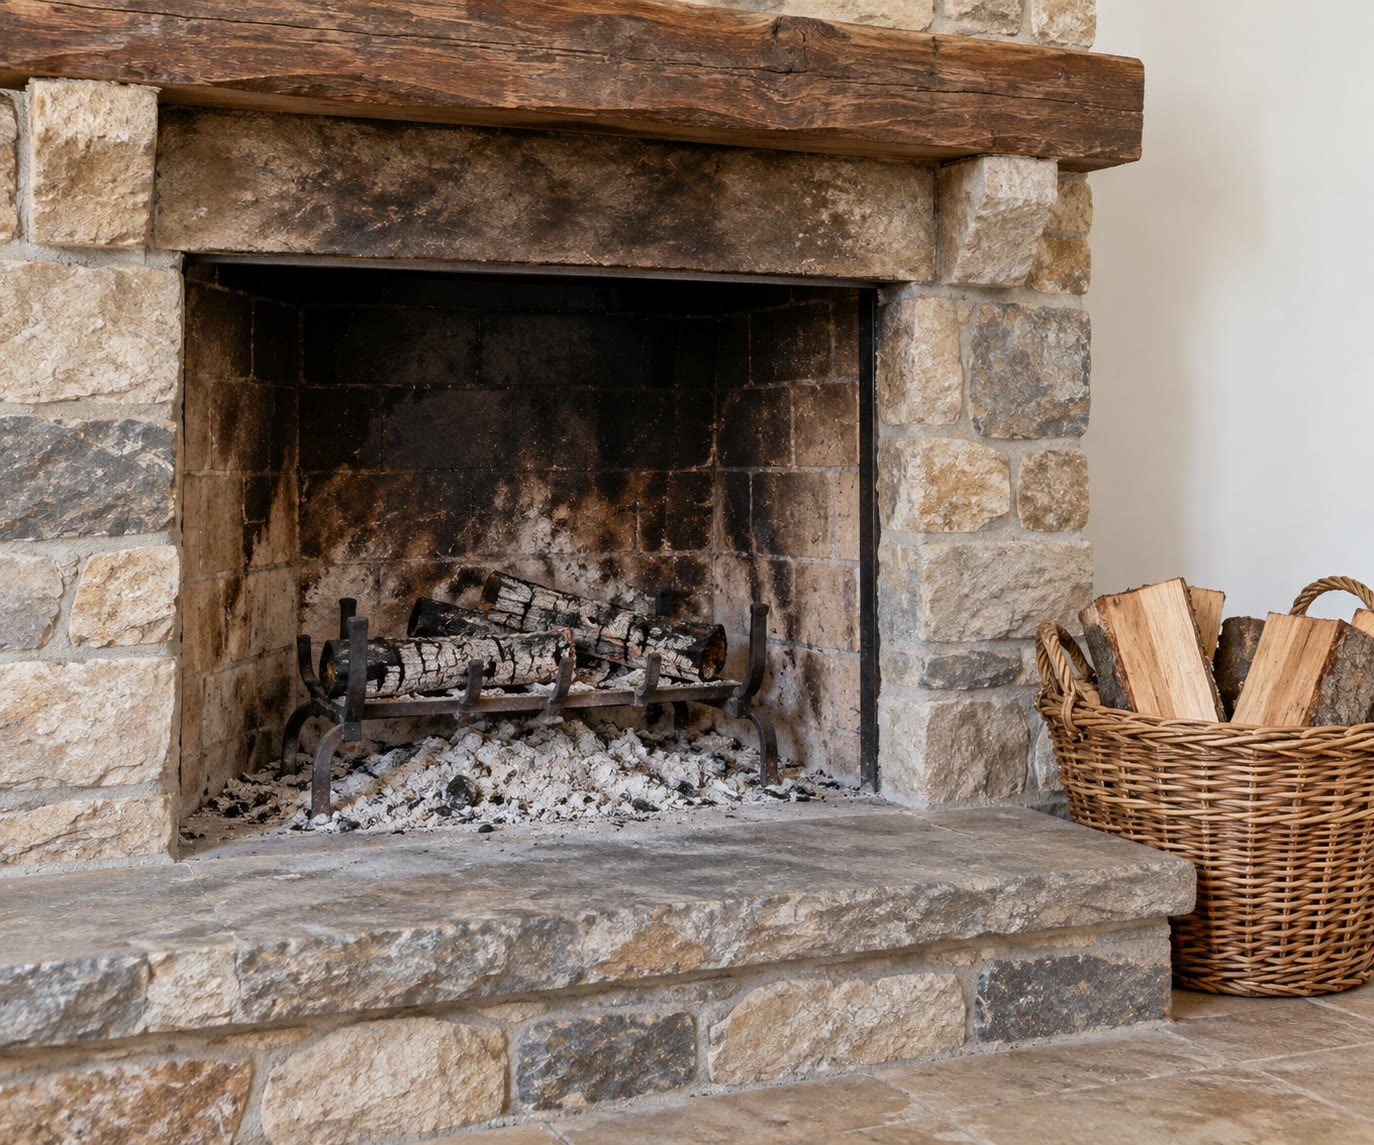
\includegraphics[width=0.5\linewidth]{images/book1/ai/g8-fireplace-ash.jpg}

{\small अगली सुबह की अँगीठी: लट्ठों में से बस थोड़ी-सी राख
बची है।}
\end{omfigure}

\section{द्रव्यमान संरक्षित रहता है}

\begin{inthelab}[बंद फ़्लास्क में अभिक्रिया को तौलना]
शिक्षक एक फ़्लास्क में थोड़ा सिरका डालते हैं, उसकी गर्दन पर चढ़ाए गए गुब्बारे
में खाने का सोडा रखते हैं, फिर पूरे को एक तुला पर रखते हैं: \qty{212.4}{g}।
गुब्बारे को उठाया जाता है ताकि सोडा सिरके में गिर जाए: \omterm{def:g6:pure-substances-and-mixtures:mixture}{मिश्रण} में सनसनाहट
होती है और बनी हुई गैस से गुब्बारा फूल जाता है। तुला अब भी
\qty{212.4}{g} दिखाती है। यही अभिक्रिया खुले फ़्लास्क में, बिना गुब्बारे के,
द्रव्यमान ``खो'' देती है: गैस कमरे में निकल जाती है।
\end{inthelab}

\begin{omfigure}
\begin{tikzpicture}[font=\small, scale=1.15]
  % closed flask
  \pic[transform shape] at (0,0) {balance};
  \pic[transform shape] at (0,0.8) {erlenmeyer={0.25}{omWater!80}};
  \fill[red!55, draw=red!60!black] (0,4.05) ellipse (0.5 and 0.62);
  \fill[red!55] (-0.3,3.45) rectangle (0.3,3.6);
  \node[anchor=north, align=center] at (0,-0.1) {बंद: गैस गुब्बारे\\ में रहती है};
  \node[anchor=west, font=\footnotesize] at (1.25,0.3) {\qty{212.4}{g}};
  % open flask
  \pic[transform shape] at (4,0) {balance};
  \pic[transform shape] at (4,0.8) {erlenmeyer={0.25}{omWater!80}};
  \foreach \y in {3.6,3.95,4.3} \draw[->, black!45, decorate,
    decoration={snake, amplitude=0.6pt, segment length=4pt}] (4,\y) -- (4,\y+0.3);
  \node[anchor=north, align=center] at (4,-0.1) {खुला: गैस निकल जाती है,\\ पाठ्यांक घटता है};
  \node[anchor=west, font=\footnotesize] at (5.25,0.3) {\qty{211.9}{g}};
\end{tikzpicture}

{\small वही अभिक्रिया, तौली गई। बंद फ़्लास्क में द्रव्यमान नहीं बदलता; खुले
फ़्लास्क में गैस निकल जाती है और तुला कम
दिखाती है।}
\end{omfigure}

\begin{definition}[द्रव्यमान संरक्षण]\label{def:g8:balanced-equations:conservation}
\emph{द्रव्यमान संरक्षण}\index{द्रव्यमान संरक्षण} वह नियम है कि
\omterm{def:g7:chemical-reactions:reaction}{रासायनिक अभिक्रिया} में बने उत्पादों का कुल द्रव्यमान खपत हुए \omterm{def:g7:chemical-reactions:reactant}{अभिकारकों} के कुल
द्रव्यमान के बराबर होता है। न कुछ खोता है, न कुछ
बनता है; द्रव्य केवल रूप बदलता है।
\end{definition}

\begin{example}[लट्ठा, ठीक से तौला गया]\label{ex:g8:balanced-equations:log}
अगर \omterm{def:g4:what-a-fire-needs:burning}{जलते} लट्ठे को और उसके द्वारा \omterm{def:g4:air-a-mixture-of-gases:air}{वायु} से ली गई ऑक्सीजन को पहले तौला जा
सकता, और राख, कार्बन डाइऑक्साइड और जलवाष्प को बाद में, तो दोनों योग बराबर
होते। राख हल्की है क्योंकि ज़्यादातर उत्पाद गैसें हैं जो चिमनी से ऊपर
चली जाती हैं।
\end{example}

\begin{history}[लावोज़िए सब कुछ तौलते हैं, 1770 का दशक--1789]
आंत्वान-लोरां लावोज़िए ने हर अभिक्रिया से पहले और बाद में हर पदार्थ को तौलने
का नियम बना लिया, और वह भी बंद पात्रों में, ताकि कोई गैस न निकल सके न
अंदर आ सके। उन्होंने दिखाया कि धातुएँ जंग लगने या \omterm{def:g4:what-a-fire-needs:burning}{जलने} पर \omterm{def:g4:air-a-mixture-of-gases:air}{वायु} से कुछ लेकर
भारी हो जाती हैं --- वह ऑक्सीजन थी, जिसका नाम उन्होंने ही रखा --- और 1789 में
कहा कि किसी अभिक्रिया में न कुछ बनता है, न कुछ खोता है। उनकी पत्नी,
मारी-आन पोल्ज़ लावोज़िए, उनके साथ काम करती थीं, प्रयोगों को दर्ज करती थीं
और उनकी पुस्तक के लिए उपकरणों के चित्र बनाती थीं।
\end{history}

\begin{omfigure}
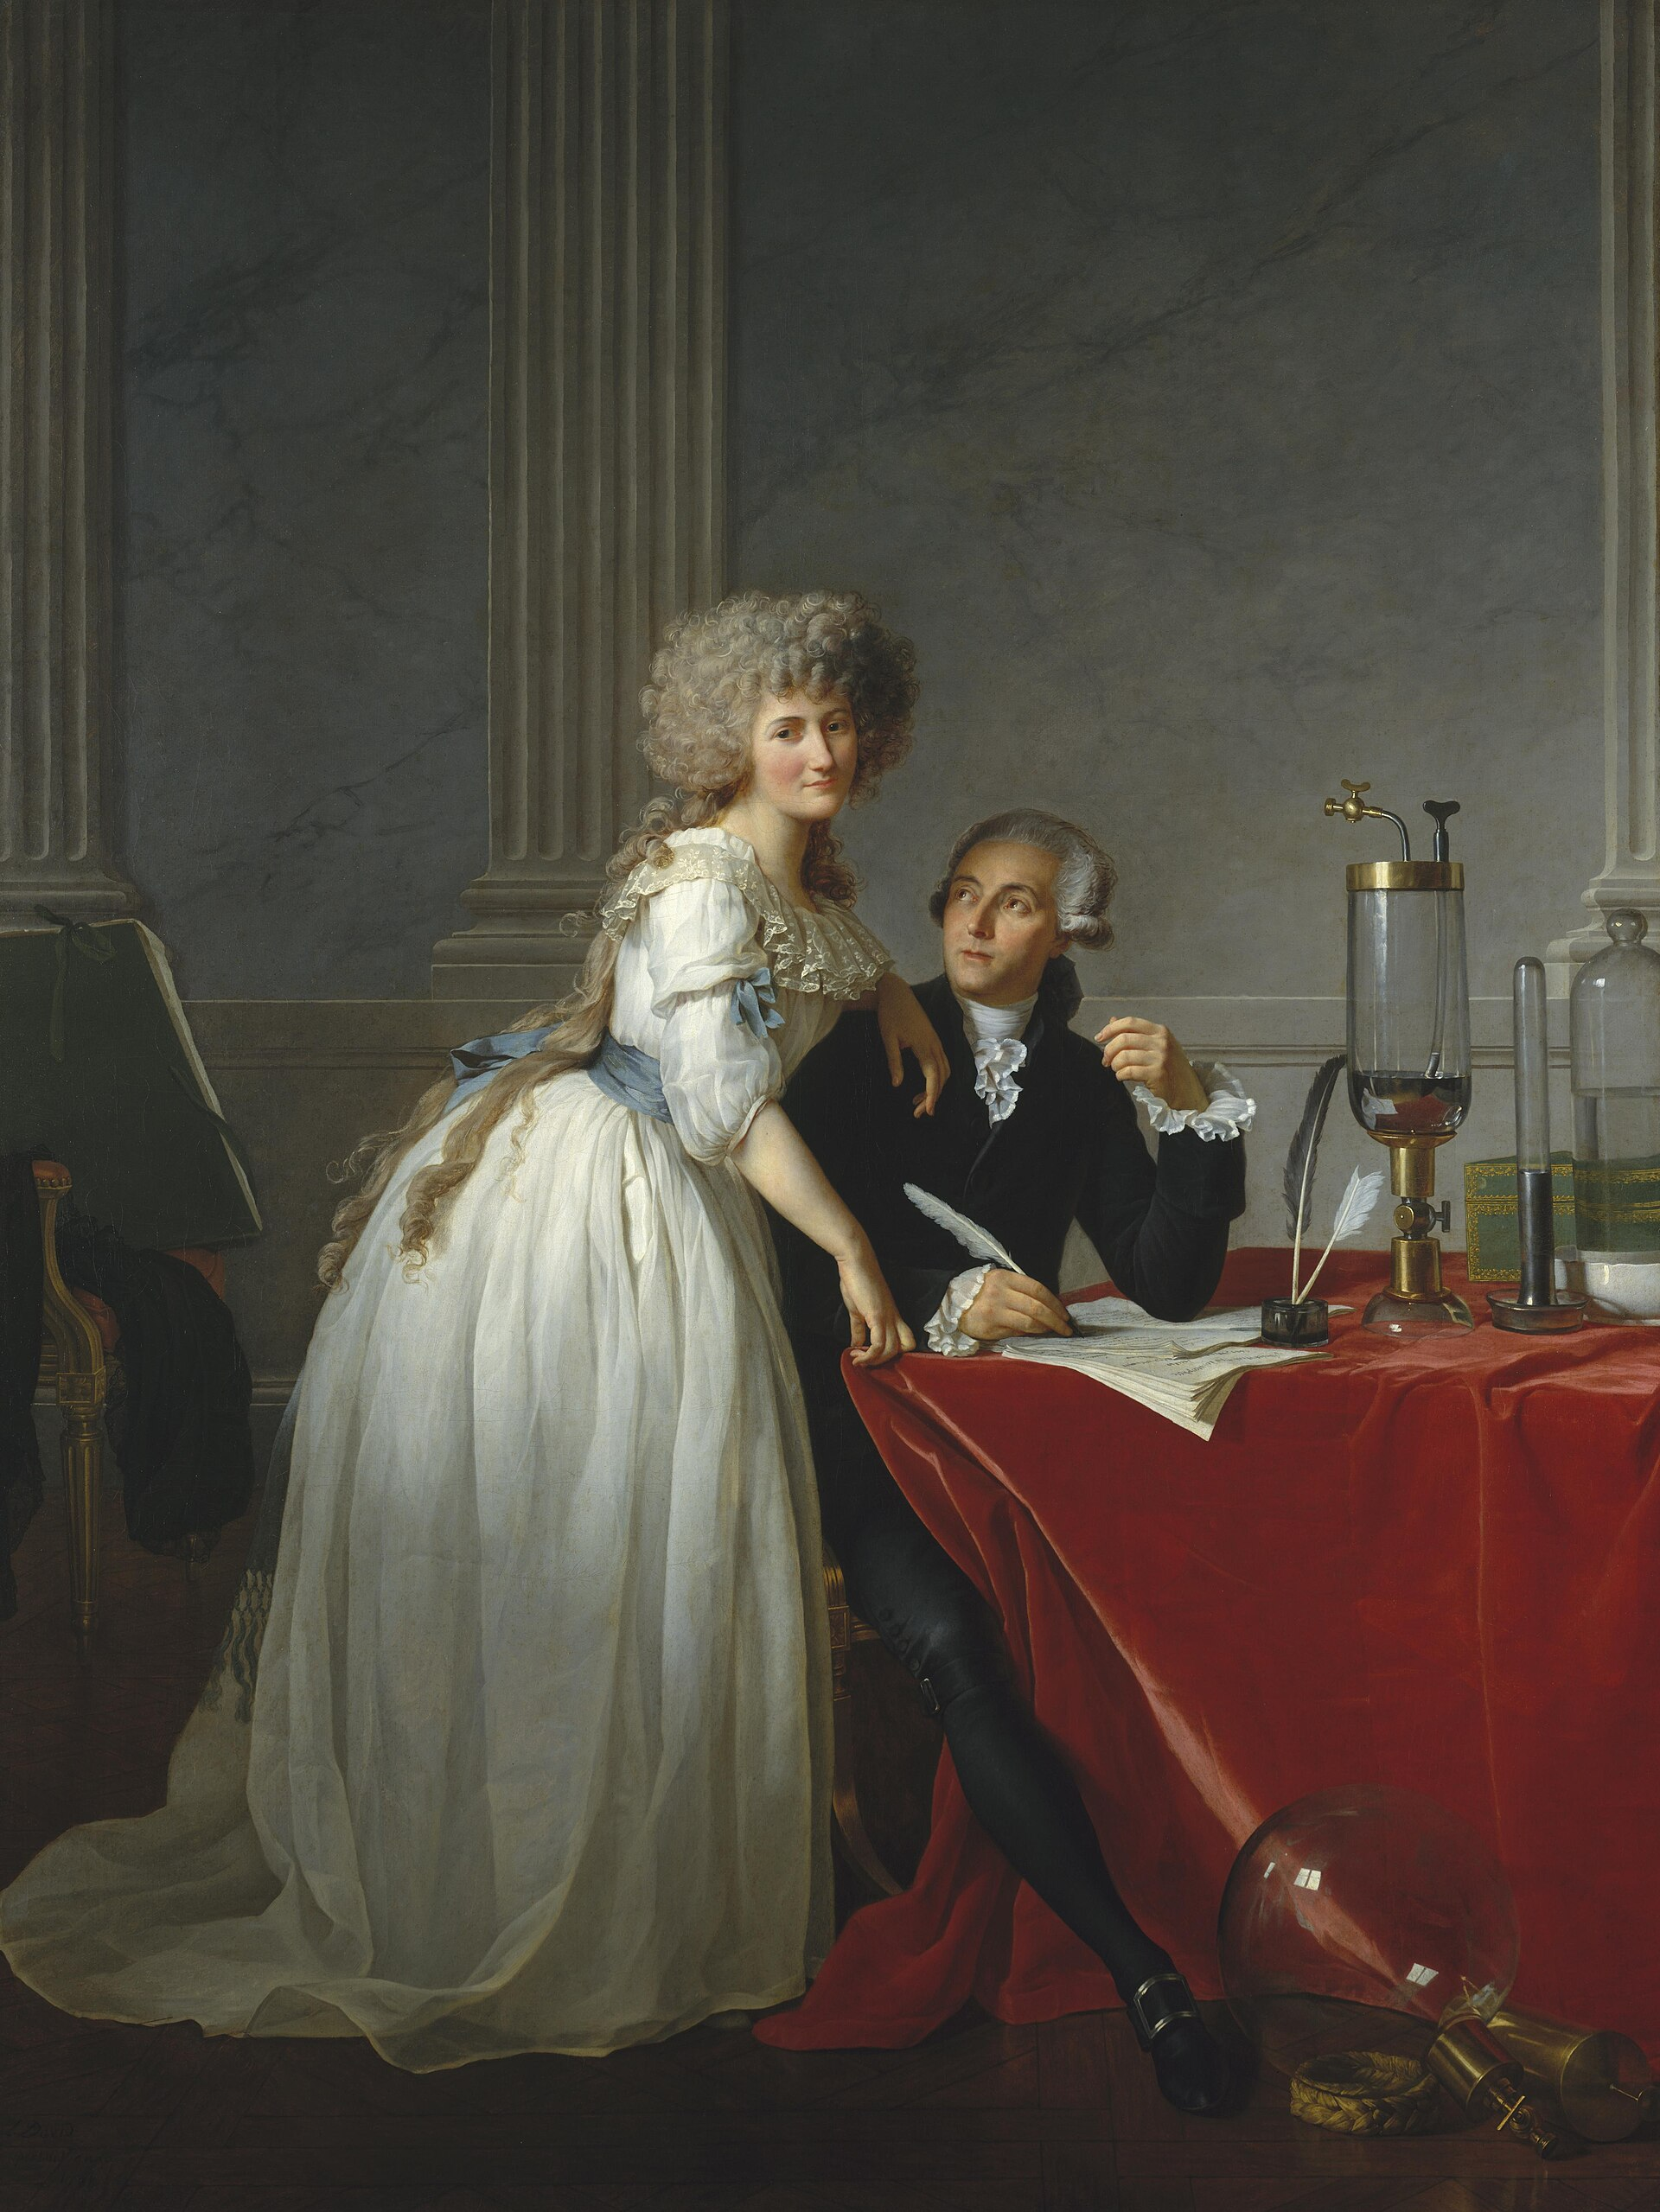
\includegraphics[width=0.3\linewidth]{images/book1/lavoisier.jpg}

{\small आंत्वान-लोरां लावोज़िए और मारी-आन पोल्ज़ लावोज़िए, चित्रकार
ज़ाक-लुई दाविद, 1788।}
\end{omfigure}

\section{द्रव्यमान संरक्षित क्यों रहता है}

\begin{proposition}[परमाणु संरक्षित रहते हैं, इसलिए द्रव्यमान संरक्षित रहता है]\label{prop:g8:balanced-equations:why}
अभिक्रिया में \omterm{def:g7:atoms-and-molecules:atom}{परमाणु} केवल नए ढंग से व्यवस्थित होते हैं: \omterm{def:g7:chemical-reactions:reactant}{अभिकारकों} का हर \omterm{def:g7:atoms-and-molecules:atom}{परमाणु}
उत्पादों में फिर मिलता है। हर \omterm{def:g7:atoms-and-molecules:atom}{परमाणु} अपना द्रव्यमान बनाए रखता है।
इसलिए कुल द्रव्यमान बदल नहीं सकता।
\end{proposition}

\begin{example}[लोहा जिसका द्रव्यमान बढ़ता है]\label{ex:g8:balanced-equations:iron}
तुला पर रखी खुली तश्तरी में \omterm{def:g4:what-a-fire-needs:burning}{जलाई} गई स्टील ऊन भारी हो जाती है: लोहे के
\omterm{def:g7:atoms-and-molecules:atom}{परमाणु} \omterm{def:g4:air-a-mixture-of-gases:air}{वायु} से ली गई ऑक्सीजन के \omterm{def:g7:atoms-and-molecules:atom}{परमाणुओं} से जुड़ गए हैं, और बने हुए आयरन
ऑक्साइड का भार लोहे और उस ऑक्सीजन के बराबर है। तुला पर \omterm{def:g4:air-a-mixture-of-gases:air}{वायु} से भरे बंद
जार में \omterm{def:g4:what-a-fire-needs:burning}{जलाने} पर पूरे का द्रव्यमान नहीं बदलता: ऑक्सीजन पहले से
जार के भीतर थी।
\end{example}

\section{रासायनिक समीकरण}

\begin{definition}[रासायनिक समीकरण]\label{def:g8:balanced-equations:equation}
\emph{रासायनिक समीकरण}\index{रासायनिक समीकरण} किसी अभिक्रिया को
सूत्रों से लिखता है: बाईं ओर \omterm{def:g7:chemical-reactions:reactant}{अभिकारकों} के सूत्र, $+$ से जुड़े हुए,
फिर एक तीर, और दाईं ओर उत्पादों के सूत्र। हर सूत्र के आगे एक संख्या
हो सकती है। समीकरण
\emph{संतुलित समीकरण}\index{संतुलित समीकरण} होता है जब हर प्रकार का
\omterm{def:g7:atoms-and-molecules:atom}{परमाणु} दोनों ओर उतनी ही बार आए।
\end{definition}

\begin{definition}[रससमीकरणमितीय गुणांक]\label{def:g8:balanced-equations:coefficient}
समीकरण में किसी सूत्र के आगे लिखी संख्या उसका
\emph{रससमीकरणमितीय गुणांक}\index{रससमीकरणमितीय गुणांक} है: यह
अभिक्रिया में भाग लेने वाले उस स्पीशीज़ के \omterm{def:g7:atoms-and-molecules:molecule}{अणुओं} (या दूसरे कणों) को गिनता है।
गुणांक 1 लिखा नहीं जाता।
\end{definition}

\begin{notation}[अवस्था-संकेत]\label{not:g8:balanced-equations:states}
सूत्र के बाद कोष्ठक में लिखा अक्षर उसकी भौतिक अवस्था बता सकता है:
(s) ठोस, (l) द्रव, (g) गैस। इस तरह \ce{H2O(l)} द्रव पानी है और
\ce{H2O(g)} जलवाष्प।
\end{notation}

\begin{example}[समीकरण पढ़ना]\label{ex:g8:balanced-equations:read}
\[
  \ce{CH4(g) + 2O2(g) -> CO2(g) + 2H2O(l)}
\]
इस तरह पढ़ा जाता है: मेथेन का एक \omterm{def:g7:atoms-and-molecules:molecule}{अणु} और ऑक्सीजन के दो \omterm{def:g7:atoms-and-molecules:molecule}{अणु} अभिक्रिया करके कार्बन
डाइऑक्साइड का एक \omterm{def:g7:atoms-and-molecules:molecule}{अणु} और पानी के दो \omterm{def:g7:atoms-and-molecules:molecule}{अणु} देते हैं। बाईं ओर: 1 C, 4 H, 4 O।
दाईं ओर: 1 C, 4 H, $2 + 2 = 4$ O। समीकरण संतुलित है।
\end{example}

\begin{omfigure}
\begin{tikzpicture}[font=\small]
  \begin{scope}[every node/.style={font=\Large, inner sep=2pt}]
    \node (a) at (0,0) {\ce{CH4}};
    \node (p1) at (0.95,0) {$+$};
    \node (b) at (1.9,0) {\ce{2O2}};
    \node (arr) at (3.35,0) {$\longrightarrow$};
    \node (c) at (4.8,0) {\ce{CO2}};
    \node (p2) at (5.75,0) {$+$};
    \node (d) at (6.8,0) {\ce{2H2O}};
  \end{scope}
  \draw[thick, omDef] ([yshift=-2pt]a.south west) -- ++(0,-0.15) -| ([yshift=-2pt]b.south east);
  \node[below=8pt, text=black] at ($(a.south)!0.5!(b.south)$) {अभिकारक};
  \draw[thick, omProp] ([yshift=-2pt]c.south west) -- ++(0,-0.15) -| ([yshift=-2pt]d.south east);
  \node[below=8pt, text=black] at ($(c.south)!0.5!(d.south)$) {उत्पाद};
  \node[above=6pt of arr, font=\small] {``अभिक्रिया करके देते हैं''};
  \node[anchor=north west, align=left, draw=black!35, rounded corners=2pt,
    font=\small, inner sep=4pt] at (-0.3,-1.25)
    {\ce{2O2} में: आगे लिखा बड़ा 2 \textbf{गुणांक} है (दो अणु);\\
     रेखा के नीचे लिखा छोटा 2 \textbf{पादांक} है (हर अणु में दो परमाणु)।};
\end{tikzpicture}

{\small \omterm{def:g8:balanced-equations:equation}{रासायनिक समीकरण} के भाग।}
\end{omfigure}

\section{समीकरण को संतुलित करना}

\begin{method}[समीकरण को संतुलित करना]\label{met:g8:balanced-equations:balance}
\begin{enumerate}
  \item \omterm{def:g7:chemical-reactions:reactant}{अभिकारकों} और उत्पादों के सही सूत्र लिखो। बाद में कभी कोई सूत्र
        मत बदलो: \ce{H2O} को \ce{H2O2} में बदलना
        किसी दूसरे पदार्थ का वर्णन होगा।
  \item दोनों ओर हर प्रकार के \omterm{def:g7:atoms-and-molecules:atom}{परमाणु} गिनो।
  \item गुणांकों की मदद से एक बार में एक ही प्रकार के \omterm{def:g7:atoms-and-molecules:atom}{परमाणु} को संतुलित करो,
        उन \omterm{def:g7:atoms-and-molecules:atom}{परमाणुओं} से शुरू करके जो हर ओर केवल एक ही सूत्र में आते हैं;
        हाइड्रोजन और ऑक्सीजन को आख़िर के लिए छोड़ दो।
  \item फिर से गिनो; तब तक दोहराओ जब तक हर प्रकार का \omterm{def:g7:atoms-and-molecules:atom}{परमाणु} संतुलित न हो जाए।
  \item सबसे छोटी पूर्ण संख्याएँ लो।
\end{enumerate}
\end{method}

\begin{example}[हाइड्रोजन और ऑक्सीजन]\label{ex:g8:balanced-equations:water}
असंतुलित: \ce{H2 + O2 -> H2O} % ce-unbalanced-ok (the skeleton)
में बाईं ओर 2 O हैं, दाईं ओर 1। \ce{H2O} के आगे 2 लगाओ: अब दाईं ओर 4 H
हैं, इसलिए \ce{H2} के आगे 2:
\[
  \ce{2H2 + O2 -> 2H2O}.
\]
जाँच: हर ओर 4 H और 2 O।
\end{example}

\begin{example}[ऑक्सीजन में लोहे का जलना]\label{ex:g8:balanced-equations:iron-oxide}
लोहा और ऑक्सीजन आयरन ऑक्साइड \ce{Fe2O3} देते हैं। ऑक्सीजन: बाईं ओर 2,
दाईं ओर 3; सबसे छोटी उभयनिष्ठ संख्या 6 है, इसलिए 3 \ce{O2} और 2
\ce{Fe2O3}। तब दाईं ओर 4 Fe हैं, इसलिए बाईं ओर 4 Fe:
\[
  \ce{4Fe + 3O2 -> 2Fe2O3}.
\]
\end{example}

\begin{omfigure}
\begin{tikzpicture}[font=\small]
  % 2 H2
  \foreach \y in {0.45,-0.45} {
    \node[aH] (a) at (0,\y) {}; \node[aH] (b) at (0.45,\y) {};
    \begin{scope}[on background layer]\draw[bond] (a.center) -- (b.center);\end{scope}}
  \node at (1.05,0) {$+$};
  \node[aO] (a) at (1.6,0) {}; \node[aO] (b) at (2.25,0) {};
  \begin{scope}[on background layer]
    \draw[bond, line width=1.1pt] ([yshift=1.6pt]a.center) -- ([yshift=1.6pt]b.center);
    \draw[bond, line width=1.1pt] ([yshift=-1.6pt]a.center) -- ([yshift=-1.6pt]b.center);
  \end{scope}
  \draw[->, thick, omProp] (2.9,0) -- (3.9,0);
  \foreach \y in {0.5,-0.5} {
    \node[aO] (o) at (4.9,\y+0.12) {};
    \node[aH] (p) at (4.35,\y-0.28) {}; \node[aH] (q) at (5.45,\y-0.28) {};
    \begin{scope}[on background layer]
      \draw[bond] (o.center) -- (p.center); \draw[bond] (o.center) -- (q.center);
    \end{scope}}
  \node[align=center, font=\footnotesize] at (1.1,-1.35) {4 H, 2 O};
  \node[align=center, font=\footnotesize] at (4.9,-1.35) {4 H, 2 O};
  \node[font=\small] at (2.7,-2.0) {\ce{2H2 + O2 -> 2H2O}};
\end{tikzpicture}

{\small हाइड्रोजन के \omterm{def:g4:what-a-fire-needs:burning}{जलने} का \omterm{def:g8:balanced-equations:equation}{संतुलित समीकरण}, मॉडलों से बनाया गया:
हाइड्रोजन के दो \omterm{def:g7:atoms-and-molecules:molecule}{अणु} और ऑक्सीजन का एक \omterm{def:g7:atoms-and-molecules:molecule}{अणु} पानी के दो
\omterm{def:g7:atoms-and-molecules:molecule}{अणु} देते हैं।}
\end{omfigure}

\section{समीकरण को अणुओं में पढ़ना}


\begin{proposition}[संतुलित समीकरण क्या कहता है]\label{prop:g8:balanced-equations:molecules}
\omterm{def:g8:balanced-equations:equation}{संतुलित समीकरण} के गुणांक बताते हैं कि कण किस अनुपात में अभिक्रिया करते हैं
और बनते हैं। अगर समीकरण \ce{2H2 + O2 -> 2H2O} है, तो हाइड्रोजन के 200 \omterm{def:g7:atoms-and-molecules:molecule}{अणु}
ऑक्सीजन के 100 \omterm{def:g7:atoms-and-molecules:molecule}{अणुओं} के साथ अभिक्रिया करके पानी के 200 \omterm{def:g7:atoms-and-molecules:molecule}{अणु} देते हैं; ऑक्सीजन
के दस लाख \omterm{def:g7:atoms-and-molecules:molecule}{अणुओं} को हाइड्रोजन के बीस लाख \omterm{def:g7:atoms-and-molecules:molecule}{अणु} चाहिए।
\end{proposition}

\begin{example}[कैंपिंग स्टोव में प्रोपेन]\label{ex:g8:balanced-equations:propane}
प्रोपेन, \ce{C3H8}, ऑक्सीजन में जलकर कार्बन डाइऑक्साइड और पानी देती है।
पहले कार्बन: 3 C, इसलिए 3 \ce{CO2}। हाइड्रोजन: 8 H, इसलिए 4 \ce{H2O}। दाईं
ओर ऑक्सीजन: $3 \times 2 + 4 = 10$ O, इसलिए 5 \ce{O2}:
\[
  \ce{C3H8 + 5O2 -> 3CO2 + 4H2O}.
\]
प्रोपेन के हर \omterm{def:g7:atoms-and-molecules:molecule}{अणु} को ऑक्सीजन के पाँच \omterm{def:g7:atoms-and-molecules:molecule}{अणु} चाहिए।
\end{example}

\section{अभ्यास}

\begin{exercise}[$\star$]\label{exo:g8:balanced-equations:1}
\omterm{def:g8:balanced-equations:conservation}{द्रव्यमान संरक्षण} का नियम बताओ।
\end{exercise}

\begin{exercise}[$\star$]\label{exo:g8:balanced-equations:2}
\ce{3CO2} में \omterm{def:g8:balanced-equations:coefficient}{रससमीकरणमितीय गुणांक} क्या है? यह कितने कार्बन \omterm{def:g7:atoms-and-molecules:atom}{परमाणुओं}
और कितने ऑक्सीजन \omterm{def:g7:atoms-and-molecules:atom}{परमाणुओं} को दर्शाता है?
\end{exercise}

\begin{exercise}[$\star$]\label{exo:g8:balanced-equations:3}
क्या \ce{C + O2 -> CO2} संतुलित है? \omterm{def:g7:atoms-and-molecules:atom}{परमाणु} गिनकर जाँचो।
\end{exercise}

\begin{exercise}[$\star$]\label{exo:g8:balanced-equations:4}
\ce{Mg + O2 -> MgO} को संतुलित करो। % ce-unbalanced-ok (to balance)
\end{exercise}

\begin{exercise}[$\star\star$]\label{exo:g8:balanced-equations:5}
\ce{N2 + H2 -> NH3} को संतुलित करो; यह अमोनिया बनाने वाली अभिक्रिया है। % ce-unbalanced-ok (to balance)
\end{exercise}

\begin{exercise}[$\star\star$]\label{exo:g8:balanced-equations:6}
\qty{12}{g} कार्बन पूरी तरह जलकर \qty{44}{g} कार्बन
डाइऑक्साइड बनाता है। कितनी ऑक्सीजन की खपत हुई?
\end{exercise}

\begin{exercise}[$\star\star$]\label{exo:g8:balanced-equations:7}
तुला पर रखे दो फ़्लास्कों वाला चित्र देखो। खुले फ़्लास्क का पाठ्यांक क्यों
घटता है? क्या द्रव्यमान नष्ट हुआ है?
\end{exercise}

\begin{exercise}[$\star\star$]\label{exo:g8:balanced-equations:8}
\ce{CH4 + O2 -> CO2 + H2O} को चरण-दर-चरण संतुलित करो, और बताओ कि हर % ce-unbalanced-ok (to balance)
चरण में तुम किस \omterm{def:g7:atoms-and-molecules:atom}{परमाणु} को संतुलित कर रहे हो।
\end{exercise}

\begin{exercise}[$\star\star$]\label{exo:g8:balanced-equations:9}
एक छात्र \ce{H2 + O2 -> H2O} को \ce{H2 + O2 -> H2O2} लिखकर संतुलित करता है। % ce-unbalanced-ok (the student's start)
यह ग़लत क्यों है?
\end{exercise}

\begin{exercise}[$\star\star$]\label{exo:g8:balanced-equations:10}
\ce{C3H8 + 5O2 -> 3CO2 + 4H2O} की मदद से बताओ कि प्रोपेन के 20 \omterm{def:g7:atoms-and-molecules:molecule}{अणुओं} को
\omterm{def:g4:what-a-fire-needs:burning}{जलाने} के लिए ऑक्सीजन के कितने \omterm{def:g7:atoms-and-molecules:molecule}{अणु} चाहिए। पानी के कितने \omterm{def:g7:atoms-and-molecules:molecule}{अणु}
बनते हैं?
\end{exercise}

\begin{exercise}[$\star\star\star$]\label{exo:g8:balanced-equations:11}
\ce{C2H6 + O2 -> CO2 + H2O}, यानी एथेन के \omterm{def:g4:what-a-fire-needs:burning}{जलने} को संतुलित करो। (संकेत: % ce-unbalanced-ok (to balance)
एथेन को दोगुना करके देखो।)
\end{exercise}

\begin{exercise}[$\star\star\star$]\label{exo:g8:balanced-equations:12}
\qty{20.0}{g} की एक मोमबत्ती \omterm{def:g4:air-a-mixture-of-gases:air}{वायु} से भरे काँच के एक बंद डिब्बे में \omterm{def:g4:what-a-fire-needs:burning}{जलती} है,
जो एक तुला पर रखा है और कुल \qty{850.0}{g} दिखाता है। लौ बुझने पर
मोमबत्ती का भार \qty{19.6}{g} है। तुला क्या दिखाती है? समझाओ।
\end{exercise}

\section{समस्या: बंद जार में स्टील ऊन}

\begin{problem}[{सप्ताहांत समस्या --- जलता हुआ लोहा, न हिलने वाली तुला,
और वायु से ली गई ऑक्सीजन}]
\label{pb:g8:balanced-equations:1}
एक प्रयोगशाला में शिक्षक स्टील ऊन को, जो लगभग शुद्ध लोहा है, दो तरह से
जलाते हैं। पहले, एक गुच्छा तुला पर रखी खुली तश्तरी में \omterm{def:g4:what-a-fire-needs:burning}{जलाया} जाता है:
पाठ्यांक बढ़ जाता है। फिर \qty{0.28}{g} का एक गुच्छा, बिजली की चिंगारी से
सुलगाकर, तुला पर रखे \omterm{def:g4:air-a-mixture-of-gases:air}{वायु} से भरे एक बंद जार के भीतर \omterm{def:g4:what-a-fire-needs:burning}{जलाया} जाता है:
पाठ्यांक नहीं बदलता। जार में लगभग \qty{0.5}{g} ऑक्सीजन है।
ऑक्सीजन में \omterm{def:g4:what-a-fire-needs:burning}{जलता} लोहा आयरन ऑक्साइड \ce{Fe2O3} बनाता है; कम ऑक्सीजन होने पर
वह \ce{Fe3O4} भी बना सकता है।

\medskip
\noindent\textbf{भाग I --- दो तौल।}
\begin{enumerate}
  \item खुली तश्तरी में द्रव्यमान बढ़ता है। अतिरिक्त द्रव्यमान कहाँ से
        आता है?
  \item बंद जार में द्रव्यमान नहीं बदलता। समझाओ।
  \item इन दो तौलों से दिखने वाला नियम बताओ।
\end{enumerate}

\medskip
\noindent\textbf{भाग II --- दो समीकरण।}
\begin{enumerate}[resume]
  \item समीकरण \ce{Fe + O2 -> Fe2O3} को संतुलित करो। % ce-unbalanced-ok (to balance)
  \item समीकरण \ce{Fe + O2 -> Fe3O4} को संतुलित करो। % ce-unbalanced-ok (to balance)
  \item पहले समीकरण की जाँच दोनों ओर हर प्रकार के \omterm{def:g7:atoms-and-molecules:atom}{परमाणु}
        गिनकर करो।
  \item पहले समीकरण के अनुसार ऑक्सीजन के कितने \omterm{def:g7:atoms-and-molecules:molecule}{अणु} लोहे के 400 \omterm{def:g7:atoms-and-molecules:atom}{परमाणुओं} के
        साथ अभिक्रिया करते हैं?
\end{enumerate}

\medskip
\noindent\textbf{भाग III --- द्रव्यमान।}
\ce{Fe2O3} में हर \qty{7}{g} लोहे के साथ \qty{3}{g}
ऑक्सीजन जुड़ी होती है। \qty{0.28}{g} का गुच्छा पूरी तरह जलकर \ce{Fe2O3} बनता है।
\begin{enumerate}[resume]
  \item \qty{0.28}{g} लोहे के साथ कितनी ऑक्सीजन जुड़ती है?
  \item कितना आयरन ऑक्साइड बनता है?
  \item क्या जार में पर्याप्त ऑक्सीजन थी? समझाओ।
  \item ठंडा होने के बाद जार खोला जाता है, और \omterm{def:g4:air-a-mixture-of-gases:air}{वायु} तेज़ी से अंदर आती है।
        समझाओ क्यों, और बताओ कि तब तुला का पाठ्यांक कैसे बदलता है।
  \item \omterm{def:g4:what-a-fire-needs:burning}{जलती} स्टील ऊन ने जार की \omterm{def:g4:air-a-mixture-of-gases:air}{वायु} से कितनी ऑक्सीजन ली, उसका द्रव्यमान
        निकालो।
\end{enumerate}
\end{problem}
